% Flowchart regression derived from the PGF trees manual grow' semantics.
\documentclass[border=2pt]{standalone}
\usepackage{tikz}
\usetikzlibrary{trees}

\tikzset{
  stage/.style={
    draw,
    rounded corners=2pt,
    minimum width=20mm,
    minimum height=8mm,
    inner sep=2pt,
    font=\small
  },
  every edge from parent/.style={draw,thick}
}

\begin{document}
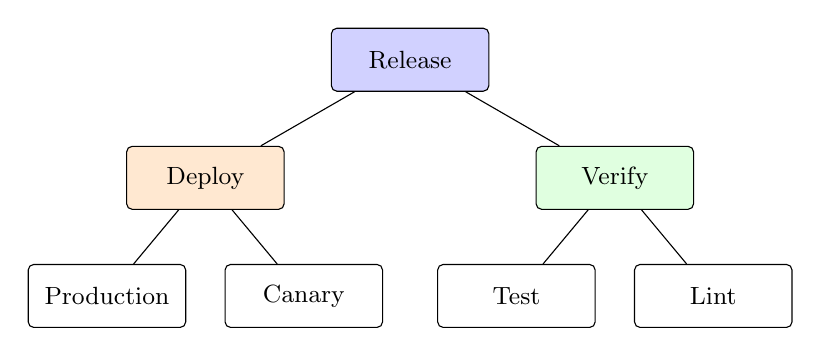
\begin{tikzpicture}[
  grow'=down,
  level distance=15mm,
  level 1/.style={sibling distance=52mm},
  level 2/.style={sibling distance=25mm}
]
  \node[stage,fill=blue!18] {Release}
    child {
      node[stage,fill=green!12] {Verify}
      child {node[stage] {Lint}}
      child {node[stage] {Test}}
    }
    child {
      node[stage,fill=orange!18] {Deploy}
      child {node[stage] {Canary}}
      child {node[stage] {Production}}
    };
\end{tikzpicture}
\end{document}
